\documentclass[12pt]{article}
\usepackage{caption}
\usepackage{float}
\usepackage{graphicx}
\usepackage{cite}
\title{\textbf{Lagrange Mean Value Theorem (LMVT)}}
\author{Sai Suddhir A B \\ \\ Roll No : AE22B013 \hspace{2cm}Github ID : parabellum20}
\date{}
\begin{document}
\maketitle
\section*{Introduction}
Joseph-Louis Lagrange(1736-1813) was one of the leaders of the movement to create a solid theory of the derivative.He tried to create his theory of the derivative around Taylor series expansions but was not entirely successful.\ \\[0.1in]
Augustin-Louis Cauchy(1789-1857), a pivotal character in building the theory of calculus, built a promising theory of calculus by building upon the works of Lagrange and others.The more generalised version of Lagrange Mean Value Theorem is the Cauchy Mean Value Theorem which goes beyond the scope of this paper. Therefore I would restrict myself to LMVT.\ 
\begin{flushleft}
\textbf{Theorem :} If the function $f(x)$ is :
\end{flushleft}
\begin{itemize}
\item Continuous on the closed interval $[a,b]$ 
\item Differentiable in the open interval $(a,b)$
\end{itemize}
\renewcommand{\thefootnote}{\Roman{footnote}}
$$\exists \hspace{0.2cm}\alpha \in (a,b) : f(b) - f(a) = f^\prime(\alpha)(b - a)\footnote[1]{Thomas, G. B. (1994). Thomas' Calculus (12th ed.). Massachusetts Institute of Technology: Pearson Education.}$$
$where \hspace{0,2cm}f^\prime(\alpha) = \frac{df}{dx}|_{x=\alpha}$ \
\\ \\[0.1cm]
\textbf{Proof :}
Let 
$$ g(x) = f(x) - \frac{f(b)-f(a)}{b-a}(x-a)$$ 
Then g(a)=g(b)=f(a). The result follows by applying Rolle's Theorem to g. -\cite{Wang2016ProofOL} \
\section*{Geometric Meaning}
\begin{figure}[H]
     \centering
     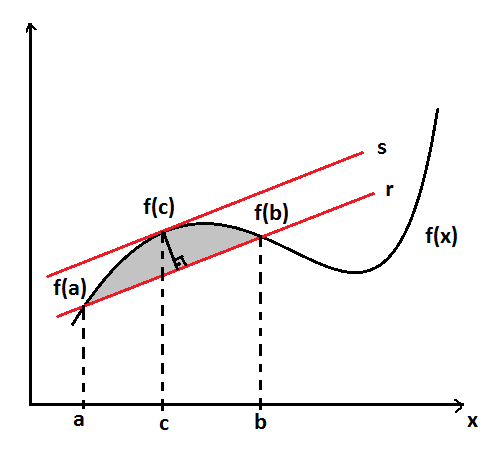
\includegraphics[scale=0.5]{LMT.png}
     \caption{Lagrange Mean Value Theorem}
\end{figure}     
Given a curve across any two points satisfying the two conditions stated by rolle's theorem , LMVT says that there exists a point in the curve where the tangent is parallel to the straight line joining the two end points. By applying the mean value theorem to the remainder term in the Taylor series, known as the Lagrange remainder or the remainder term of the Taylor polynomial, one can establish bounds and error estimates for approximating functions using Taylor polynomials.
\section*{Applications}
\begin{itemize}
    \item It is used to prove Taylor Series expansion, find the remainder term in Taylor series and establish bounds and error estimates for approximating functions using Taylor polynomials.
    \item It is used to determine the existence and uniqueness of equation roots. ~\cite{Jiang_2020}
    \item In general it is used to prove equations, inequalities and study the properties of derivates and functions. ~\cite{Jiang_2020}
\end{itemize}
\section*{Reason for choice}
Being very bad at mathematics, I had no motivation to learn deeper and explore the intricacies of the maths I had learned during JEE. To my surprise, I understood math better than other subjects during my first semester and I owe it completely to my professor who wanted to impart pure mathematical thinking to all his students. The usage of the Lagrange mean value theorem was unparalleled by any other theorem in the course he took on Multivariable Calculus. It helped me develop mathematical concepts which webbed around the LMVT and that is why I find this equation particularly beautiful.
\bibliographystyle{unsrt}
\bibliography{citation}
\end{document}